\chapter{Evaluation und Validation}
\label{ch:Eval}

In diesem Kapitel werden die Resultate der Modelle wie in \ref{sec:method_eval} beschrieben evaluiert. Zuerst wird darauf
eingegangen wie die Resultate der Modelle evaluiert werden. Weiter wird aufgeführt welche Anforderungen erreicht werden
sollten. Anschliessend wird die eigentliche Evaluation durchgeführt.

\section{Vorgehen der Evaluierung}
\label{sec:vorgehen_evaluation}

Wie bereits in \ref{sec:method_eval} beschrieben wird soll die Verteilung der Satzlänge der Ausgangssätze sowie den
Zielsätzen verglichen werden. Wie auch in \ref{sub:statistische_analyse_des_datensatz} aufgeführt werden die Stillabel $
wikipedia $ und $ klexikon $ durch ihre Satzlänge unterschieden. Für die Evaluierung wird auf den Validationsteil des
Datensatzes ein Transfer durchgeführt. Dabei werden die Sätze aus dem Stillabel $ wikipedia $ in einen Satz aus dem
Stillabel $ klexikon $ transferiert. Entsprechendes gilt für die Sätze aus dem Label $ klexikon $, welche in einen Satz
aus dem Stillabel $ wikipedia $ gewandelt werden. Für das erreichen der Anforderungen ist vorallem die Wandlung
von kürzeren Sätzen in das Labels $ klexikon $ interessant. Dies da es sich bei den Zielen der Aufgabenstellung,
\ref{sec:Aufgabenstellung-Zielsetzung}, ebenfalls um einen Transfer handelt welche eine längere Satzlänge fordert.
\newline
\newline
Um die Verteilung er Satzlängen aus den Stillabels zu vergleichen werden ca. $ 15'000 $ Sätze aus jedem Stillabel einem
Transfer unterzogen. Anschliessend werden die Anzahl Wörter des Eingabesatzes sowie des entsprechenden Ausgabesatz
verglichen. Anschliessend wird die Differenz der Länge der beiden Sätze gebildet. Es wird erwartet das der Durchschnitt
der Differenz für die Ausgabesätze grösser $ 0 $ entspricht.
\newline
\newline
Aufgrund der Resultate in \ref{sec:resultate} wurde entschieden das letzte Modell
\fullref{sub:bigger_embedding_hyperparameter} zu evaluieren. Um ebenfalls einen Vergleich zwischen den beiden Modelle
ControlGen und CrossAlign zu erhalten, wird ebenfalls das CrossAlign Modell aus
\ref{sub:weighted_hyperparameter} mit der beschriebenen Methode evaluiert. Beide evaluierten Modelle wurden auf dem
Datensatz \flqq Gekürzt\frqq trainiert.
\newline
\newline
Als Evaluierungs Datensatz wird ein Teil des Datensatz \flqq Ausgeglichen\frqq \ verwendet. Dieser beinhaltet beinhaltet
die Verteilung welche in
\fullref{sub:statistische_analyse_des_datensatz}, Abbildung \fullref{fig:distribution_both_cleaned_and_equalized}
aufgezeigt wird.

\section{Verteilung des Evaluierungs Datensatz}
\label{sec:distri_eval_data}

Die Verteilung der Sätzlängen auf dem Evaluierungs Datensatz folgt der gleichen Verteilung wie der gesamte Datensatz
\flqq Ausgeglichen\frqq. Die Verteilung der Satzlängen der beiden Stile ist in \fullref{fig:distribution_klexi_clean} und
\fullref{fig:distribution_wiki_clean} aufgezeigt. Zum Vergleich sind in den Abbildungen \ref{fig:distribution_eval_dataset_klexi}
und \ref{fig:distribution_eval_dataset_wiki} die Verteilungen der Satzlängen aus dem Validationsteil des Datensatz \flqq
Ausgeglichen\frqq \ abgebildet.

\begin{figure}[H]
    \minipage{0.45\textwidth}
      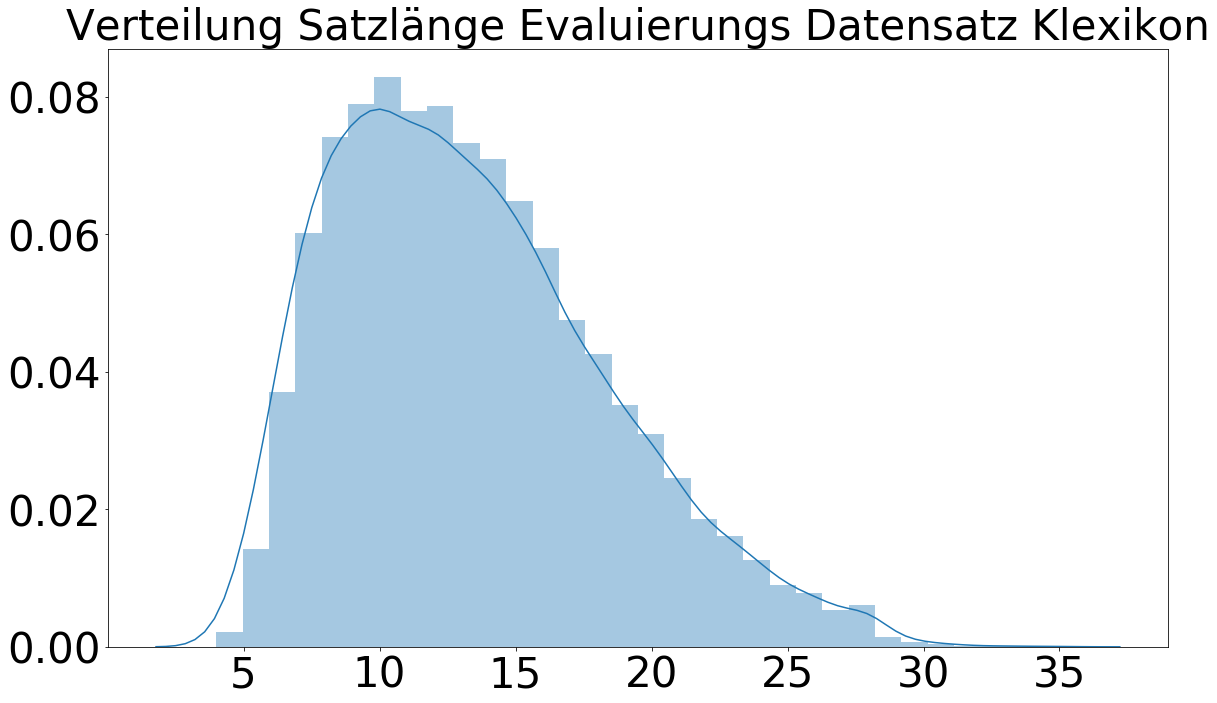
\includegraphics[width=\linewidth]{eval/distribution_eval_dataset_klexi.png}
      \caption{Verteilung Satzlänge Klexikon Evaluierungs Datensatz}\label{fig:distribution_eval_dataset_klexi}
    \endminipage\hfill
    \minipage{0.45\textwidth}
      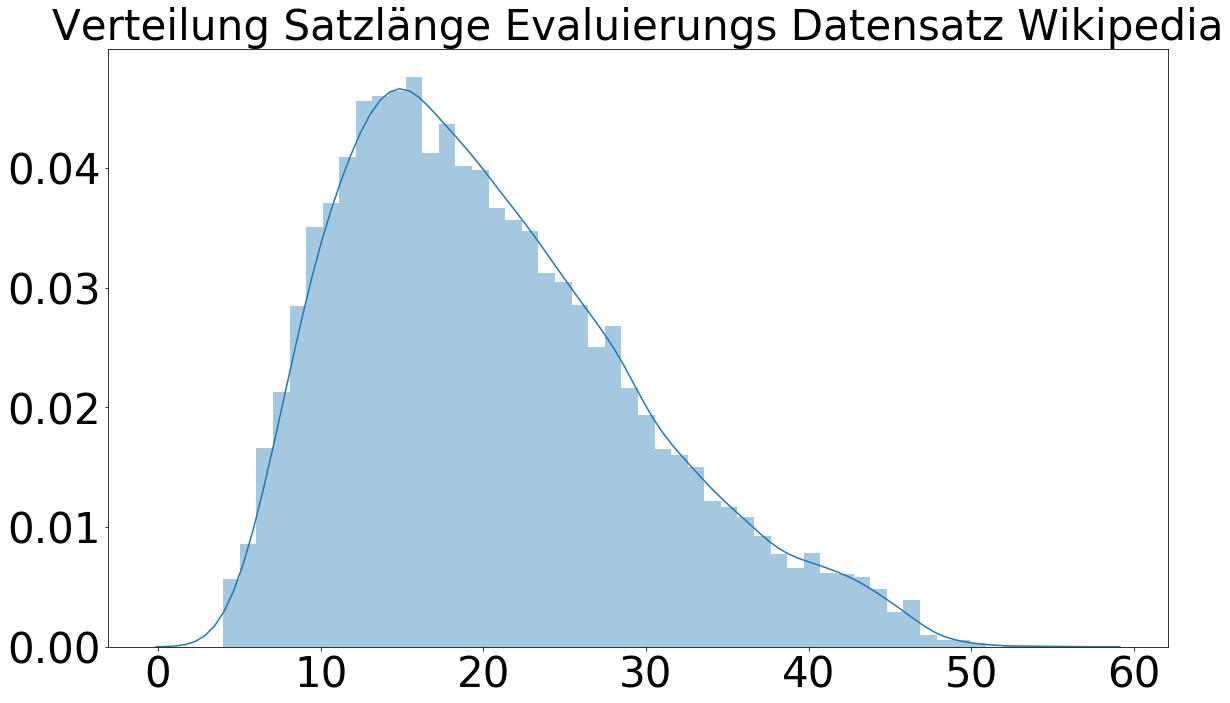
\includegraphics[width=\linewidth]{eval/distribution_eval_dataset_wiki.png}
      \caption{Verteilung Satzlänge Wikipedia Evaluierungs Datensatz}\label{fig:distribution_eval_dataset_wiki}
    \endminipage\hfill      
 \end{figure}
 \begin{table}[H]
    \centering
    \begin{tabular}{|c|c|c|c|c|c|}
      \hline
      \textbf{Datenquelle}& \textbf{25\% Quartil}& \textbf{Median}& \textbf{75\% Quartil} & \textbf{Mean} &
      \textbf{Standardabweichung}\\
      \hline
      \textbf{Klexikon}& 9 & 13 & 17 & 13.4 & 5.1\\
      \hline
      \textbf{Wikipedia}& 14 & 19 & 26 & 20.6 & 9.1\\
      \hline
    \end{tabular}
    \caption{Verteilung Evaluierungs Datensatz}
    \label{tab:distribution_eval_dataset}
  \end{table}  
\noindent
Wie in Abbildung \ref{fig:distribution_eval_dataset_klexi} und \ref{fig:distribution_eval_dataset_wiki} zu sehen ist
folgt der Evaluierungs Datensatz wie erwartet einer nahezu identischen Verteilung wie der Datensatz \flqq Ausgeglichen\frqq.

\section{Evaluierung der Modelle}
\label{sec:eval-eval}

\subsection{CrossAlign gewichtete Verlustfunktion}
\label{sec:eval-weighted-loss}

Als erstes wurde eine Evaluierung auf dem CrossAlign Modell aus \ref{sub:weighted_hyperparameter} durchgeführt.
Nachfolgend wird gezeigt wie die Verteilung der Ausgabesätze für die beiden Transfers ausfällt.

\begin{figure}[H]
    \minipage{0.45\textwidth}
      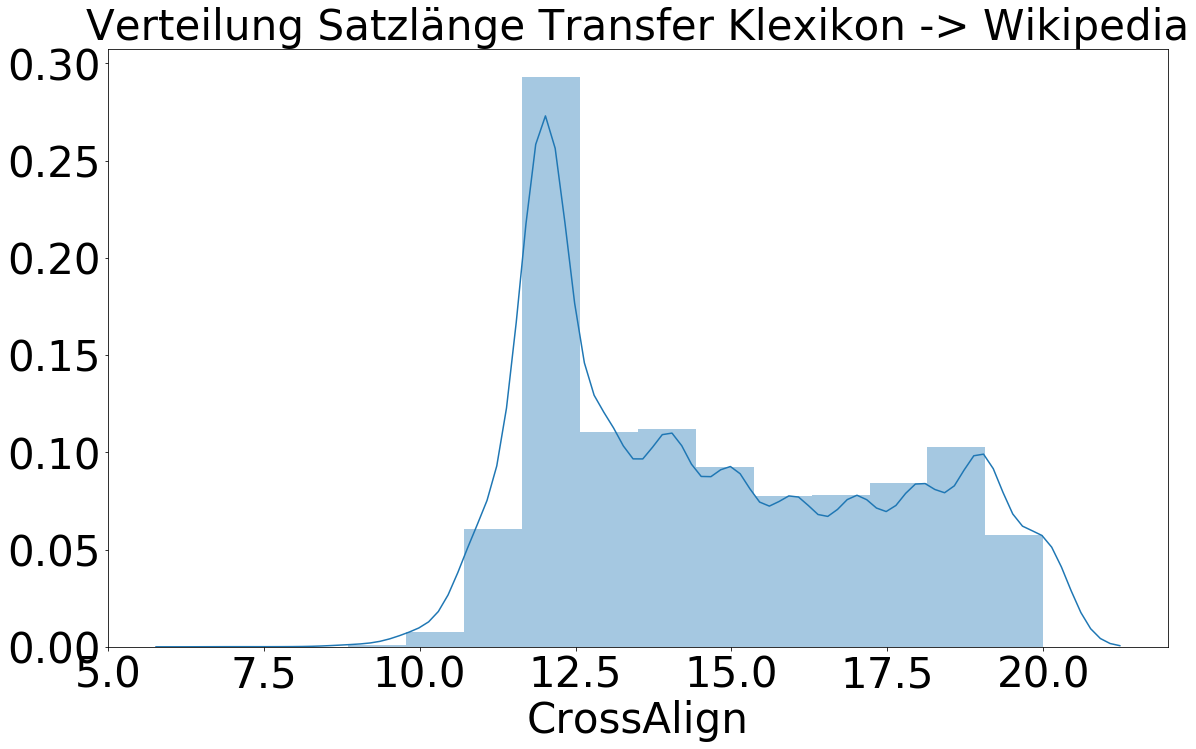
\includegraphics[width=\linewidth]{eval/crossalign/distribution_transfer_klexi_wiki_crossalign.png}
      \caption{Verteilung Satzlänge Transfer Klexikon zu Wikipedia CrossAlign}\label{fig:distribution_transfer_klexi_wiki_crossalign}
    \endminipage\hfill
    \minipage{0.45\textwidth}
      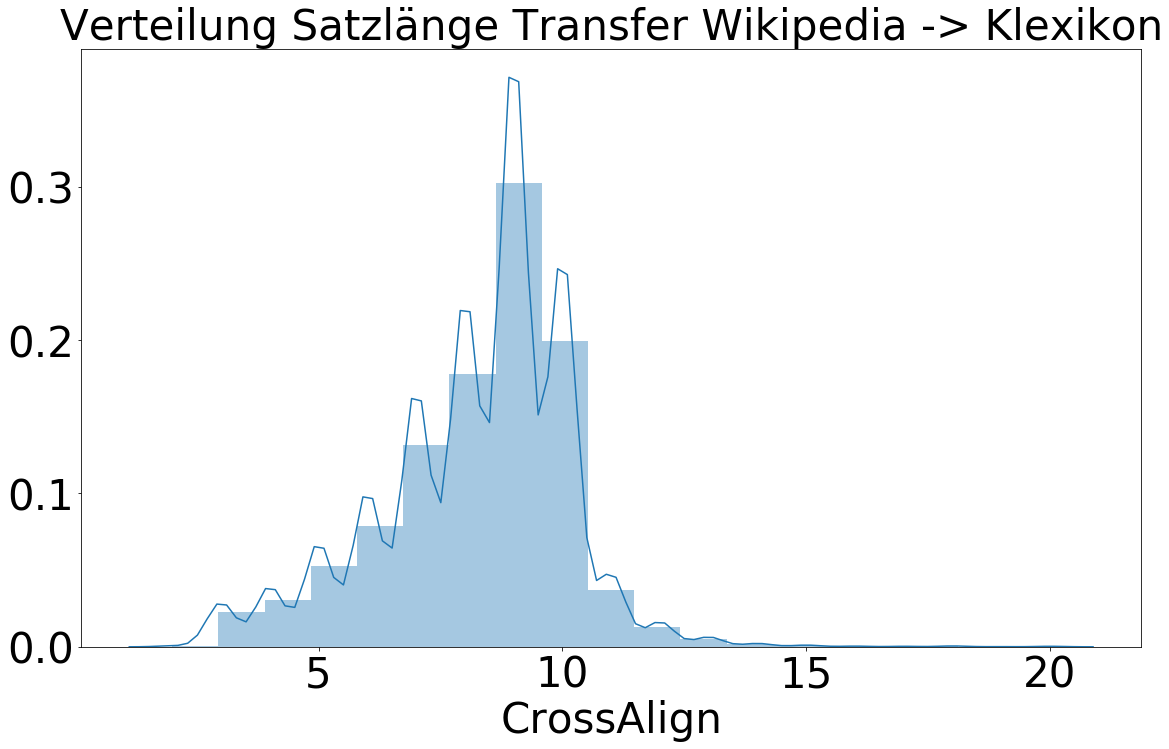
\includegraphics[width=\linewidth]{eval/crossalign/distribution_transfer_wiki_klexi_crossalign.png}
      \caption{Verteilung Satzlänge Transfer Wikipedia zu Klexikon CrossAlign}\label{fig:distribution_transfer_wiki_klexi_crossalign}
    \endminipage\hfill       
 \end{figure}
 \begin{table}[H]
    \centering
    \begin{tabular}{|c|c|c|c|c|c|}
      \hline
      \textbf{Transfer}& \textbf{25\% Quartil}& \textbf{Median}& \textbf{75\% Quartil} & \textbf{Mean} &
      \textbf{Std. Abw.}\\
      \hline
      \textbf{Klexikon -> Wikipedia}& 12 & 14 & 17 & 14.7 & 2.8\\
      \hline
      \textbf{Wikipedia -> Klexikon}& 11 & 13 & 15 & 12.7 & 2.5\\
      \hline
    \end{tabular}
    \caption{Verteilung Satzlänge Transfer CrossAlign}
    \label{tab:distribution_transfer_crossalign}
  \end{table} 
\noindent
\newline
Wie aus den Grafiken \ref{fig:distribution_transfer_klexi_wiki_crossalign} und
\ref{fig:distribution_transfer_wiki_klexi_crossalign} und der Tabelle \ref{tab:distribution_transfer_crossalign}
entnommen werden kann findet durchaus für beide Transfer eine Verschiebung der Verteilungen statt. Dabei scheint der
Transfer vom Stil $ wikipedia $ in den Stil $ klexikon $ besser zu funktionieren. Der Transfer von $ klexikon $ zu $
wikipedia $ ändert die Verteilung ebenfalls, diese ist jedoch weniger nahe bei einer Gaussverteilung.
\newline
\newline
Als nächstes soll auf die Differenz der Länge des Eingabe- und des Ausgabesatzes eingegangen werden.

\begin{figure}[H]
    \minipage{0.45\textwidth}
      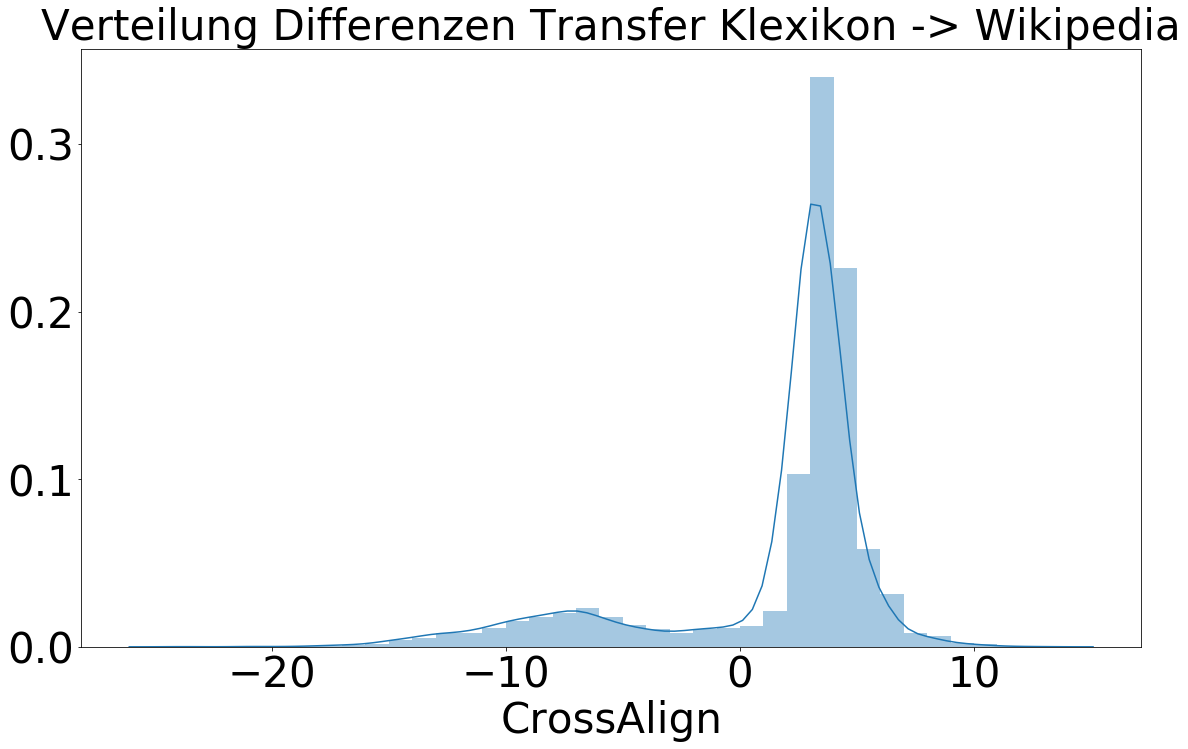
\includegraphics[width=\linewidth]{eval/crossalign/distribution_differences_klexi_wiki_crossalign.png}
      \caption{Verteilung Differenz Klexikon -> Wikipedia CrossAlign}\label{fig:distribution_diff_klexi_wiki_crossalign}
    \endminipage\hfill
    \minipage{0.45\textwidth}
      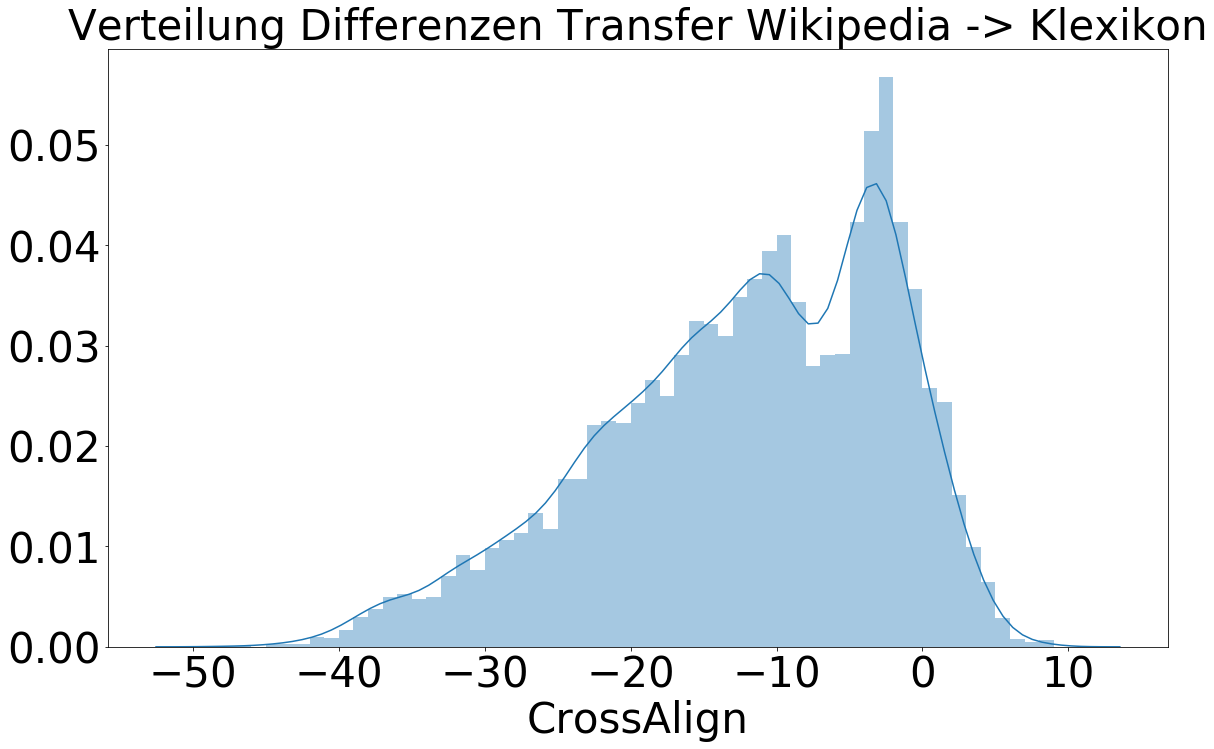
\includegraphics[width=\linewidth]{eval/crossalign/distribution_differences_wiki_klexi_crossalign.png}
      \caption{Verteilung Differenz Wikipedia -> Klexikon CrossAlign}\label{fig:distribution_diff_wiki_klexi_crossalign}
    \endminipage\hfill      
 \end{figure}
 \begin{table}[H]
    \centering
    \begin{tabular}{|c|c|c|c|c|c|}
      \hline
      \textbf{Transfer}& \textbf{25\% Quartil}& \textbf{Median}& \textbf{75\% Quartil} & \textbf{Mean} &
      \textbf{Std. Abw.}\\
      \hline
      \textbf{Klexikon -> Wikipedia}& 2 & 3 & 4 & 1.35 & 4.8\\
      \hline
      \textbf{Wikipedia -> Klexikon}& -19 & -11 & -4 & -12.39 & 9.9\\
      \hline
    \end{tabular}
    \caption{Verteilung Differenzen Transfer CrossAlign}
    \label{tab:difference_transfer_crossalign}
  \end{table}  
\noindent
\newline
In den Differenzen zeigen sich die Erkenntnisse welche auch aus den Verteilungen in Abbildungen
\ref{fig:distribution_transfer_klexi_wiki_crossalign} und \ref{fig:distributin_transfer_wiki_klexi_crossalign}
ersichtlich sind. Beide Transfers verlängern, beziehungsweise verkürzen, den Satz. Der Transfer von $ wikipedia $ zu $
klexikon $ weist im Durchschnitt, siehe Mean in Tabelle \ref{tab:difference_transfer_crossalign}, eine höhere Differenz
auf als der Transfer von $ klexikon $ zu $ wikipedia $. Diese Aussage wird jedoch durch die ebenfalls höhere
Standardabweichung relativiert.

\subsection{ControlGen mit grösseren Dimensionen}
\label{sec:eval-higher-dimensions}

Es wird nun das Modell ControlGen evaluiert welches für den Style Transfer vielversprechende Werte aufzeigt, siehe
\fullref{sub:bigger_embedding_hyperparameter}. Ebenfalls wird hier zuerst auf die Verteilung der Ausgabesätze
eingegangen und anschliessend die Differenzen untersucht.


\begin{figure}[H]
    \minipage{0.45\textwidth}
      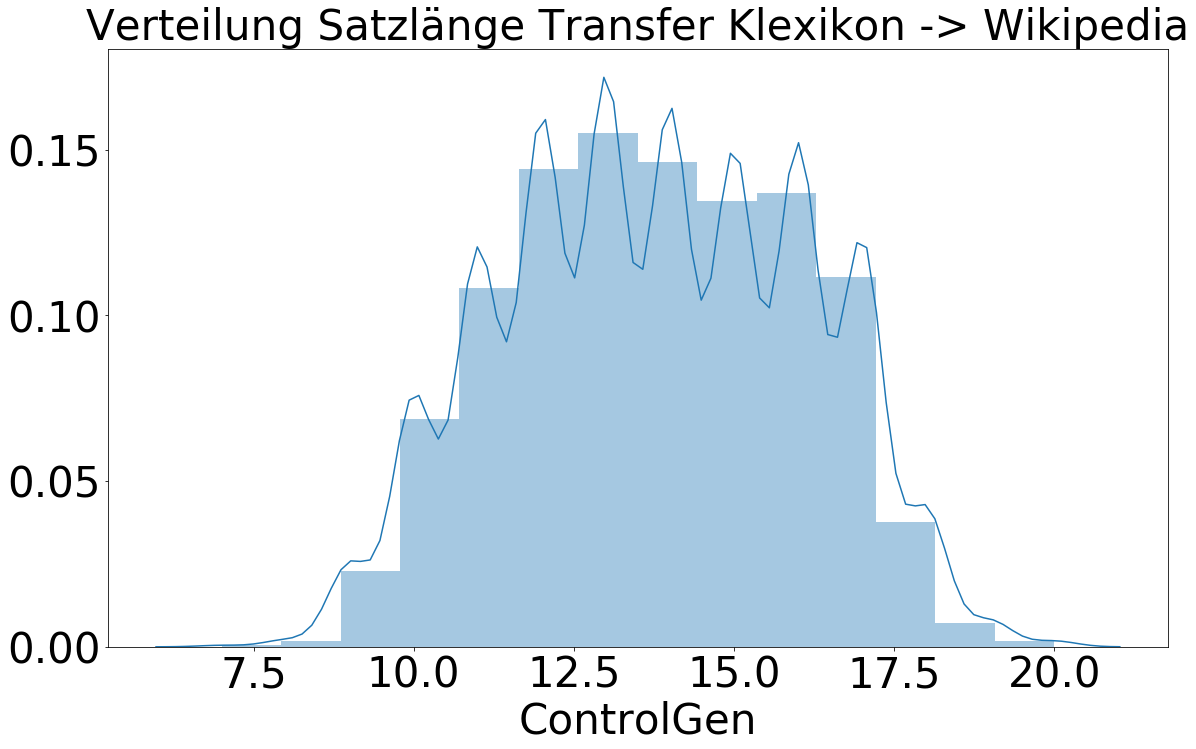
\includegraphics[width=\linewidth]{eval/controlgen/distribution_transfer_klexi_wiki_controlgen.png}
      \caption{Verteilung Satzlänge Transfer Klexikon zu Wikipedia ControlGen}\label{fig:distribution_transfer_klexi_wiki_controlgen}
    \endminipage\hfill
    \minipage{0.45\textwidth}
      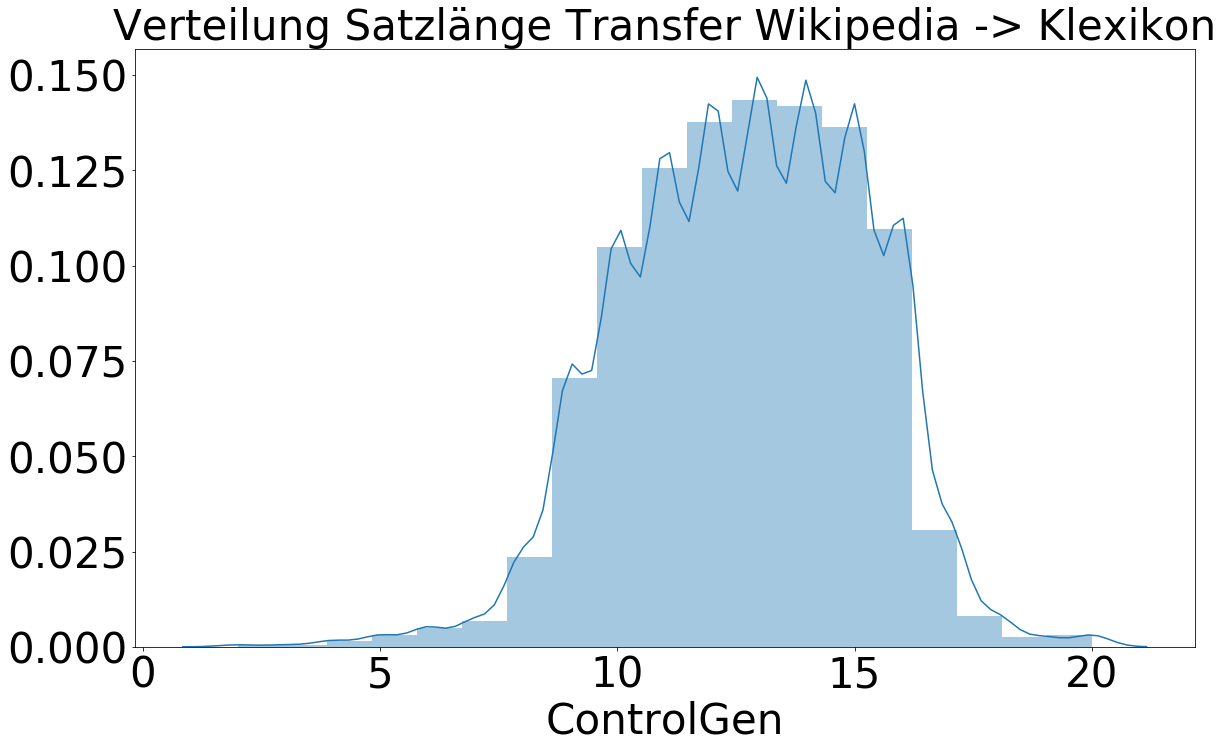
\includegraphics[width=\linewidth]{eval/controlgen/distribution_transfer_wiki_klexi_controlgen.png}
      \caption{Verteilung Satzlänge Transfer Wikipedia zu Klexikon ControlGen}\label{fig:distribution_transfer_wiki_klexi_controlgen}
    \endminipage\hfill       
 \end{figure}
 \begin{table}[H]
    \centering
    \begin{tabular}{|c|c|c|c|c|c|}
      \hline
      \textbf{Transfer}& \textbf{25\% Quartil}& \textbf{Median}& \textbf{75\% Quartil} & \textbf{Mean} &
      \textbf{Std. Abw.}\\
      \hline
      \textbf{Klexikon -> Wikipedia}& 12 & 14 & 16 & 13.8 & 2.3\\
      \hline
      \textbf{Wikipedia -> Klexikon}& 11 & 13 & 15 & 12.7 & 2.5\\
      \hline
    \end{tabular}
    \caption{Verteilung Satzlänge Transfer ControlGen}
    \label{tab:distribution_transfer_controlgen}
  \end{table} 
\noindent
\newline
Auch für das ControlGen kann eine Verschiebung der Verteilung beobachtet werden. Diese fällt jedoch weniger stark aus
als beim Modell CrossAlign. Das ControlGen Modell scheint dabei die Ausgabesätze in einen kleinen Bereich zu zwängen.
Dieser befinet sich für den Transfer von $ klexikon $ zu $ wikipedia $ bei $ 12 $ bis $ 16 $. Für den Transfer $
klexikon $ zu $ wikipedia $ bei $ 11 $ bis $ 15 $. Dies entspricht den 25\%- und 75\% Quartilen der Verteilung. Dies
kann ebenfalls aus der Tabelle \ref{tab:distribution_transfer_controlgen} entnommen werden. 
\newline
\newline
Interessant ist dabei der Rückschluss auf Resultate des Trainings, siehe \fullref{sub:bigger_embedding_hyperparameter}.
Dort weis das Modell eine höhe Genauigkeit für den Style Transfer aus. Obwohl die Längen der Ausgabesätze sich minimal
unterscheidet.

\begin{figure}[H]
    \minipage{0.45\textwidth}
      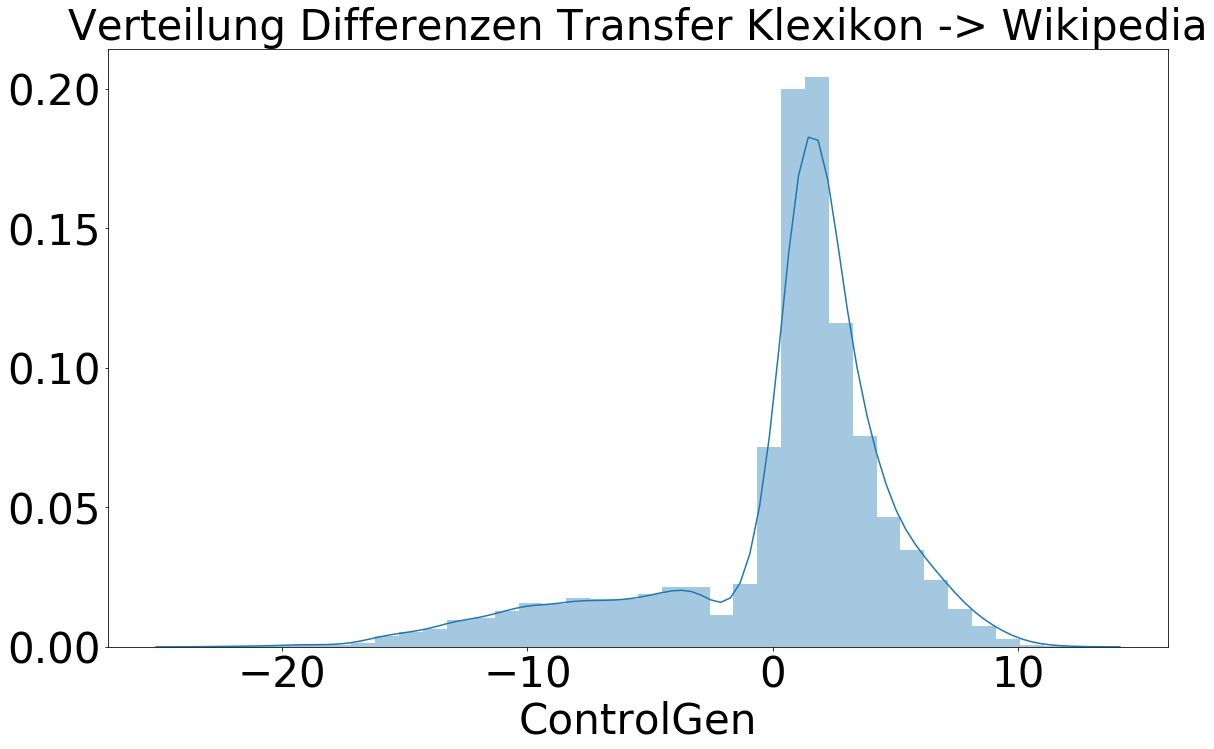
\includegraphics[width=\linewidth]{eval/controlgen/distribution_differences_klexi_wiki_controlgen.png}
      \caption{Verteilung Differenz Klexikon -> Wikipedia ControlGen}\label{fig:distribution_transfer_klexi_wiki_controlgen}
    \endminipage\hfill
    \minipage{0.45\textwidth}
      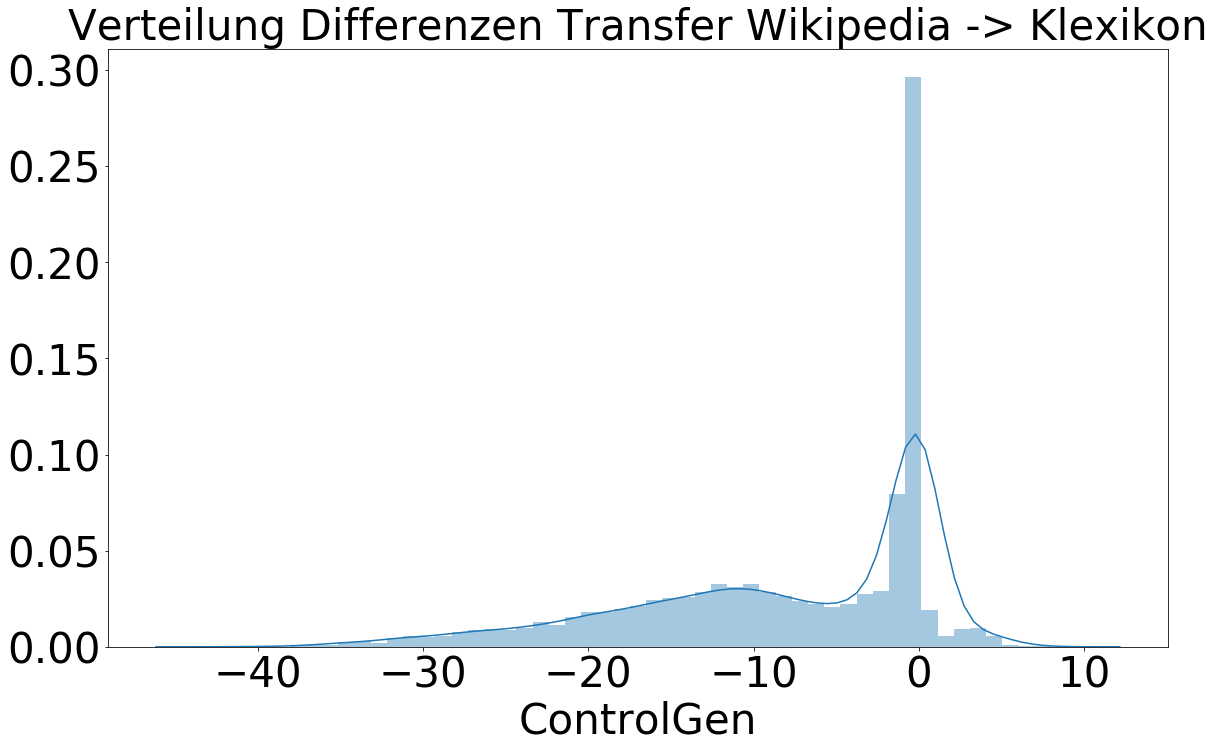
\includegraphics[width=\linewidth]{eval/controlgen/distribution_differences_wiki_klexi_controlgen.png}
      \caption{Verteilung Differenz Wikipedia -> Klexikon ControlGen}\label{fig:distribution_transfer_wiki_klexi_controlgen}
    \endminipage\hfill      
 \end{figure}
 \begin{table}[H]
    \centering
    \begin{tabular}{|c|c|c|c|c|c|}
      \hline
      \textbf{Transfer}& \textbf{25\% Quartil}& \textbf{Median}& \textbf{75\% Quartil} & \textbf{Mean} &
      \textbf{Std. Abw.}\\
      \hline
      \textbf{Klexikon -> Wikipedia}& 0 & 2 & 3 & 0.45 & 4.9\\
      \hline
      \textbf{Wikipedia -> Klexikon}& -14 & -5 & 0 & -7.88 & 9.14\\
      \hline
    \end{tabular}
    \caption{Verteilung Differenzen Transfer ControlGen}
    \label{tab:distribution_eval_diff_controlgen}
  \end{table}  
\noindent
\newline
Auch hier zeigen die Differenzen ein ähnliches Bild wie beim \fullref{sec:eval-weighted-loss}. Der Durschnitt, siehe
Tabelle \ref{tab:distribution_eval_diff_controlgen} für das Modell ControlGen fällt jedoch kleiner aus als für das
CrossAlign. Jedoch weist auch für dieses Modell der Transfer von $ wikipedia $ zu $ klexikon $ eine höhere
Standardabweichung auf.

\subsection{Evaluierung der Ausgabesätze}
\label{sec:eval_output}

Wie bereits in \fullref{sec:abschliessende_problemdefinition} beschrieben bestand der Fokus darauf die Länge der Sätze
zu ändern, anstelle der Verständlichkeit der Sätze. Auch der \gls{BLEU} Scores der Resultate der Trainings, siehe
\ref{sec:resultate}, kann erkennt werden, dass die Verständlichkeit der Sätze gering ist. Dennoch soll zur
Vervollständingung an einem Beispiel aufgezeigt werden, wie der Transfer der Modelle ausgeführt wurde. Das Wort
\textit{<unk>} markiert ein Wort welches sich nicht im Vokabular des Models befindet, siehe \fullref{sub:base_model}.
\newline
\newline
\textbf{Eingabesatz Stillabel $ klexikon $}
\newline
\textit{dort sollte Varus die Grenze gegen die Germanen bewachen .}
\newline
\newline
\textbf{Ausgabesatz Stillabel $ wikipedia $}
\newline
\textit{dort sollte Ricken die Nationalversammlung gegen die Lage Populationen Leistungen auf Lage , <unk> .}
\newline 
\newline
Wie am Beispiel gesehen werden kann, ist der transferierten Sätze unverständlich und bezieht sich kaum bis gar nicht auf
den Kontext des Eingabesatzes. Daher wird auf eine genauere Evaluation der Qualität der Ausgabesätze verzichtet. Dies
auch wie bereits erwähnt aufgrund des Fokus die Satzlänge zu verändern.

\section{Vergleich mit Anforderungen}
\label{sec:VergleichAnforderungen}

Im Kapitel \fullref{ch:Eval} wurde gezeigt, dass durchaus eine Veränderung der Verteilung statt gefunden hat. Die
Verteilungen ändern sich jedoch zu gering um sich der Verteilung des Zielstils anzupassen. Damit konnte mit dem
\gls{NST} das Ziel, die Verteilung des Zielstils zu erhalten nicht erreicht werden. 
\newline
\newline
Da die Modelle kein Vokabular aus dem Bereich von Zwischen- und Arbeitzeugnissen kennen, sowie der Transfer,
wie in \fullref{sec:eval_output} gezeigt, keine zufriedenstellende Resultate liefert, wurde auf ein Transfer der
Textbausteine des Auftraggebers verzichtet.



